\title{Recap Big data: architectures and data analytics (01QYDOV)}
\author{Jacopo Nasi\\
        Computer Engineer\\
        Politecnico di Torino}
\date{II Period - 2018/2019\\\bigskip\bigskip\today}

\documentclass[12pt]{article}
\usepackage[utf8]{inputenc}
\usepackage[english]{babel}
\usepackage{geometry}
\usepackage{indentfirst} % First line indent
\usepackage{mathtools}
\usepackage{wrapfig}
\usepackage[usenames, dvipsnames]{color}
\usepackage{float}
\usepackage{amssymb}
\usepackage{ifsym}
\usepackage{listings}
\usepackage{multicol}

% Misure Documento
\geometry{ a4paper, total={170mm,257mm},left=35mm, right=35mm, top=35mm, bottom=35mm }

\begin{document}

\begin{figure}
  \centering
  
\includegraphics[width=10cm]{images/polito.pdf}
\end{figure}

\maketitle


\newpage
\tableofcontents

\newpage
{\noindent \Large \textbf{License}\bigskip}

This work is licensed under a Creative Commons Attribution-NonCommercial-ShareAlike 3.0 Unported License.\\
You are free:
\begin{itemize}
  \item \textbf{to Share}: to copy, distribute and transmit the work
  \item \textbf{to Remix}: to adapt the work
\end{itemize}
Under the following conditions:
\begin{itemize}
  \item \textbf{Attribution}: you must attribute the work in the manner specified by the author or licensor (but not in any way that suggests that they endorse you or your use of the work)
  \item \textbf{Noncommercial}: you may not use this work for commercial purposes.
  \item \textbf{Share Alike}: if you alter, transform, or build upon this work, you may distribute the resulting work only under the same or similar license to this one.
\end{itemize}

\noindent More information on the Creative Commons website (http://creativecommons.org).

\begin{figure}[h!]
  \centering
  
\includegraphics[width=3cm]{images/license.png}
\end{figure}

{\noindent \Large \textbf{Acknowledgments}\bigskip}

Questo breve riepilogo non ha alcuno scopo se non quello di agevolare lo studio di me stesso, se vi fosse di aiuto siete liberi di usarlo.\\
Le fonti su cui mi sono basato sono quelle relative al corso offerto (\textbf{Big data: architectures and data analytics (01QYDOV)}) dal Politecnico di Torino durante l'anno accademico 2018/2019.\\
Non mi assumo nessuna responsabilità in merito ad errori o qualsiasi altra cosa. Fatene buon uso!
\newpage

\section{Introduction}
The amount of data increases every days, to analyze them, system must scale according. All these systems must deal with computation capabilities, network bandwidth and failures. A good pratice to solve problems is the parallelizations, a single-node architectiure cannot solve, in reasonable time, the request of these days. For these reasons, nowadays, clusters (fig.\ref{fig:cluster}) are pretty common.
\begin{figure}[H]
  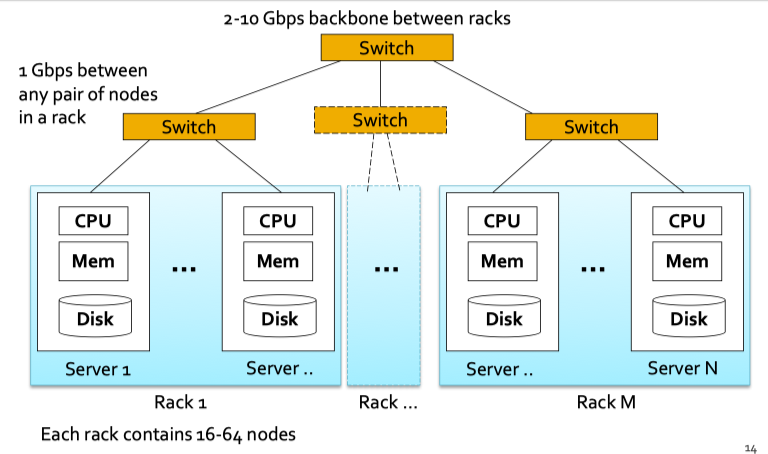
\includegraphics[width=\linewidth]{images/cluster.png}
  \caption{Cluster Architecture}
  \label{fig:cluster}
\end{figure}
The main characteristics are:
\begin{itemize}
  \item \textbf{Scalability}: Increase number of users, amount of datas, complexity of problems
  \begin{itemize}
    \item Scale \textbf{UP}: More power/resources for a single-node
    \item Scale \textbf{OUT}: Add more nodws to the cluster
  \end{itemize}
\end{itemize}

\section{Apache Hadoop}
Scalable fault-tolerant distributed system for Big Data: Distributed Data Storage, Distributed Data Processing, etc...
Is an Open Source project under Apache license. Is used by a lot of main IT companies all around the world.\\
The core of the structure are:
\begin{itemize}
  \item \textbf{Distributed BD Processing Infrastructure} (MapReduce):
  \begin{itemize}
    \item High-level abstraction view: Not require to take care of scheduling and synchronizations
    \item Fault Tolerant: Node and task are automatically managed
  \end{itemize}
  \item \textbf{HDFS} (Hadoop Distributed File System):
  \begin{itemize}
    \item Fault-Tolerant
    \item High availability distributed storage
  \end{itemize}
\end{itemize}
The paradigm of MapReduce will not be illustrated, in figure \ref{fig:mapreduce} a sample of the process during the word count problem.
\begin{figure}[H]
  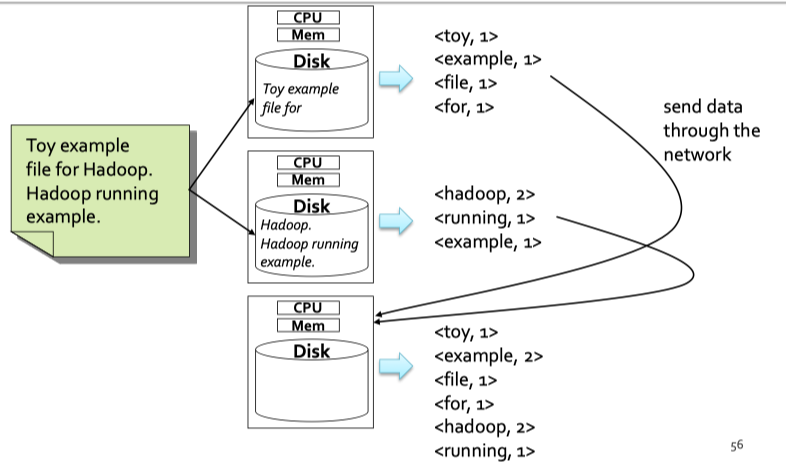
\includegraphics[width=\linewidth]{images/mapreduce.png}
  \caption{MapReduce Example}
  \label{fig:mapreduce}
\end{figure}

\subsection{Structure of a program}
The project is divided in different parts:
\begin{itemize}
  \item Driver: Coordinators of the jobs
  \item Mapper: Class for the Map part
  \item Reducer: Class implementing the Reduce part
\end{itemize}
There are also other important terms:
\begin{itemize}
  \item Job: Execution of a MapReduce code over a dataset
  \item Task: Execution of a Map task or a Reducer task on a slice of data
\end{itemize}
The workflow of a project is similar to the following one:
\begin{figure}[H]
  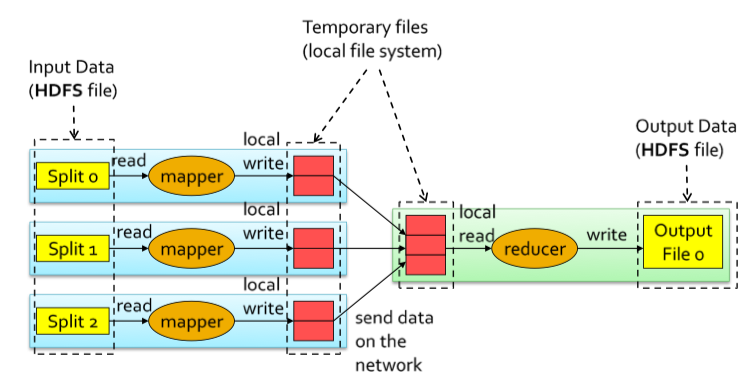
\includegraphics[width=\linewidth]{images/wf.png}
  \caption{MapReduce Workflow in Hadoop}
  \label{fig:wf}
\end{figure}

\subsection{Data Types}
Hadoop make use of its own basic data types:
\begin{itemize}
  \item Text: Like Java string
  \item IntWritable: Like java integer
  \item LongWritable
  \item FloatWritable
\end{itemize}
Also the data for the input and output has its own type:
\begin{itemize}
  \item TextInputFormat (Lines)
  \item KeyValueTextInputFormat (2 Fields)
  \item SequenceFileInputFormat (Binary)
\end{itemize}
Also the output have similar formats.\\
Is also possible to define personalized data types, these also the usage of more complex values. To use them, is required, to implements the \textit{org.apache.hadoop.io.Writable} interface and its methods, in particular:
\begin{itemize}
  \item write()
  \item readFields()
\end{itemize}
also the method toString is important, in order to generate the value to be emit with the pair.

\subsection{Combiner and Counters}
In standard MapReduce applications the (key,value) pairs emitted by mappers are sent to the reducers through the newtork. In some case, a sort of "pre-aggreations" could be useful to improve performances and reduce the amount of data shared on the network.\\
An example with the word count problem with clarify the usage of combiners.
\begin{figure}[H]
  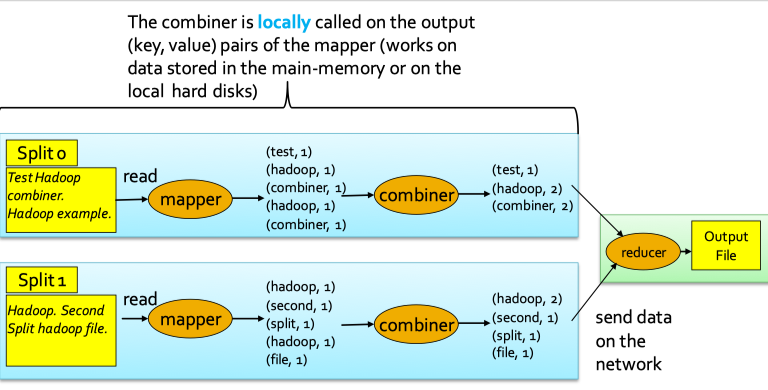
\includegraphics[width=\linewidth]{images/combiners.png}
  \caption{Example of combiner usage}
  \label{fig:cobiners}
\end{figure}
Is an instance of the Reducer class, that implements a pre-reduce phase, characterized by the reduce() method. It process (key, [list of value]) and emits (key, value). It runs on the cluster.\\
Combiners and be also exploited by in-mapper solutions, by initialize a set of in-mapper variables during the instance of the Mapper. They are created by using setup/cleanup methods.\\
Hadoop provides a set of vasic, built-in, counters to store some statistics about jobs, mappers and reducers. Also some ad-hoc, user-defined, counters can be defined. They can be used by the exploting enum Java types, and increment by using the following code:
\begin{center}
  \textit{context.getCounter(countername).increment(val ue);}
\end{center}

\subsection{Configurations}
Is possible to define some properties shared among the different part (M,C,R), they must be defined in the driver using the following syntax:
\begin{center}
  \textit{conf.set("property-name", "value");}
\end{center}
and they can be retrived in the Mapper and/or Reducer phase by using:
\begin{center}
  \textit{context.getConfiguration().get("property-name");}
\end{center}

\subsection{Map-only job}
In some cases everything can be achived using the Mapper phase only. Of course, Hadoop, allows the execution of this kind of jobs. Everything is achived by setting the number of reducers task to zero. \textbf{Not setting this value can generate problems during the executions}.

\subsection{Setup and Cleanup methods}
Are two optional methods to be invoked in the Mapper class, one at the start (Setup()) and the other at the end, both invoked one time for each mapper.

\subsection{Patterns}
Common patterns to solve problems. The following are know as \textbf{Summarization Patterns}:
\paragraph{Numerical Summarizations} group records/objects by a key filed and calculate a numberical aggregate (avg, min, max, std deviations, etc...). Are used to provide a top-level view of large input data sets. They are used to analyze, by domain experts, trends or anomalies.\\
The phase:
\begin{itemize}
  \item \textbf{Mappers}: Key is used to define groups, Value for computing aggregate statistics
  \item \textbf{Reducers}: Receive a set of numerical values for each "group-by" key and compute the final stats
  \item \textbf{Combiners}: Used to speed-up the process
\end{itemize}

\paragraph{Inverted Index Summarizations} the goal is to build an index from the input data to support faster search or data enrichment.
\begin{itemize}
  \item \textbf{Mappers}: Key is the set of fields to index (a keyword), Value is a unique identifier of the objects to associare with each "keyword"
  \item \textbf{Reducers}: Receive a set of identifiers for each keyword and simply concatenate them
  \item \textbf{Combiners}: Normally NOT used
\end{itemize}

\paragraph{Counting with Counters} the goal is to compute count summarizations of data sets. Also this solutions can be used to identify trends and anomalies.
\begin{itemize}
  \item \textbf{Mappers}: Process each input record and increment a set of counters
\end{itemize}
This pattern can be achived by using also MapOnly jobs, the result are directly printed by the Driver of the application.\\

The following are know as \textbf{Filtering Patterns}:
\paragraph{Filtering} has the goal to filter out input records that are not of interest and keep the others, in order to focusing only on the records of interest. The pourpose is to reduce the set of the data for the analysis.
\begin{itemize}
  \item \textbf{Mappers}: Output one pair for each record that satisfies the enforced rule
  \item \textbf{Reducers}: Almost useless
\end{itemize}

\paragraph{Top K} is select a small set of top K record according to a ranking function. Used to focusing only on the most important (for the ranking function) values.
\begin{itemize}
  \item \textbf{Mappers}: Each mapper initializes an in-mapper top K list (small), cleanup emits the pairs after the complete scan
  \item \textbf{Reducers}: a Single Instance compute the final top k list by merging the local lists
\end{itemize}

\paragraph{Distinct} it finds a unique set of values/records, prune the duplicates.
\begin{itemize}
  \item \textbf{Mappers}: Emit one (key, null) pair for each input record
  \item \textbf{Reducers}: Emit one (key, null) pair for each input (key, list of values) pair
\end{itemize}

\subsection{Multiple Inputs/Outputs}
Hadoop allows the user to implements different input and/or outputs, it could be useful in some case. The input differentiation is achieved by using the addInputPath() method, the output one is achieved with addNamedOutput() method.

\subsection{Distributed Cache}
Some application need to share and cache (small) read-only files to performa efficently their tasks. These files should be accessible by all nodes of the cluster in an efficient way. The Distributed Cache is a facility provided by the Hadoop-based MapReduce framework to cache files.
These files are specified in the Driver, during the initialization of the job, Hadoop create a local copy of the shared/cached files in all nodes which are used to execute some tasks of the job, the cache file is then read by the Mapper, usually in the setup method.
Save with:
\begin{center}
  job.\textbf{addCacheFile}(new Path("hdfsPath").toUri());
\end{center}
And it is retived by using:
\begin{center}
  URI[] urisCachedFiles = context.\textbf{getCacheFiles()};
\end{center}

% \subsection{Data Organization Patterns}
% Slide set #11

\end{document}
